\begin{center}\large\textbf{Readings: 11.1-11.6 and 11.9-11.11 pg 463 - 515 and 529 - 539}\\
\normalsize \end{center}
\large \hlinewd{2pt}
~\\

\textbf{Motivating Example}\\
(Taken from Probabilitiy and Statistics, Devore)  Soil and sediment adsorption, the extent to which chemicals collect in a condensed form on the surface, is an important characteristic influencing the effectiveness of pesticides and various agricultural chemicals.  A study was done on 13 soil samples that measured $Y$ = phosphate adsorption index, $X_1$ = amount of extractable aluminum, and $X_2$ = amount of extractable iron.  The data are given below:
\begin{center}
\begin{tabular}{ccc}
Adsorption & Aluminum & Iron\\
\hline
4 &13& 61\\
18&21&175\\
14&24&111\\
18&23&124\\
26&64&130\\
26&38&173\\
21&33&169\\
30&61&169\\
28&39&160\\
36&71&244\\
65&112&257\\
62&88&333\\
40&54&199\\
\end{tabular}
\end{center}

\textbf{MLR model for two quantitative explantory variables:}\\
For observation $i$ we can use the model
$$Y_i = \beta_0 + \beta_1 X_{i1} + \beta_2 X_{i2} + E_{i}$$

\newpage

For clarity we can write the model for each subject
\begin{eqnarray*}
Y_{1} &=& \beta_0 + \beta_1 X_{11} + \beta_2 X_{12} + E_{1}  \\
Y_{2} &=& \beta_0 + \beta_1 X_{21} + \beta_2 X_{22} + E_{2}  \\
\vdots & = & \vdots \\
Y_{13} &=& \beta_0 + \beta_1 X_{13,1} + \beta_2 X_{13,2} + E_{13}  
\end{eqnarray*}
Generally our model is 
$$Adsorption = \beta_0+\beta_1Aluminum+\beta_2Iron+Experimental~Error$$
~\\~\\~\\
\begin{center}
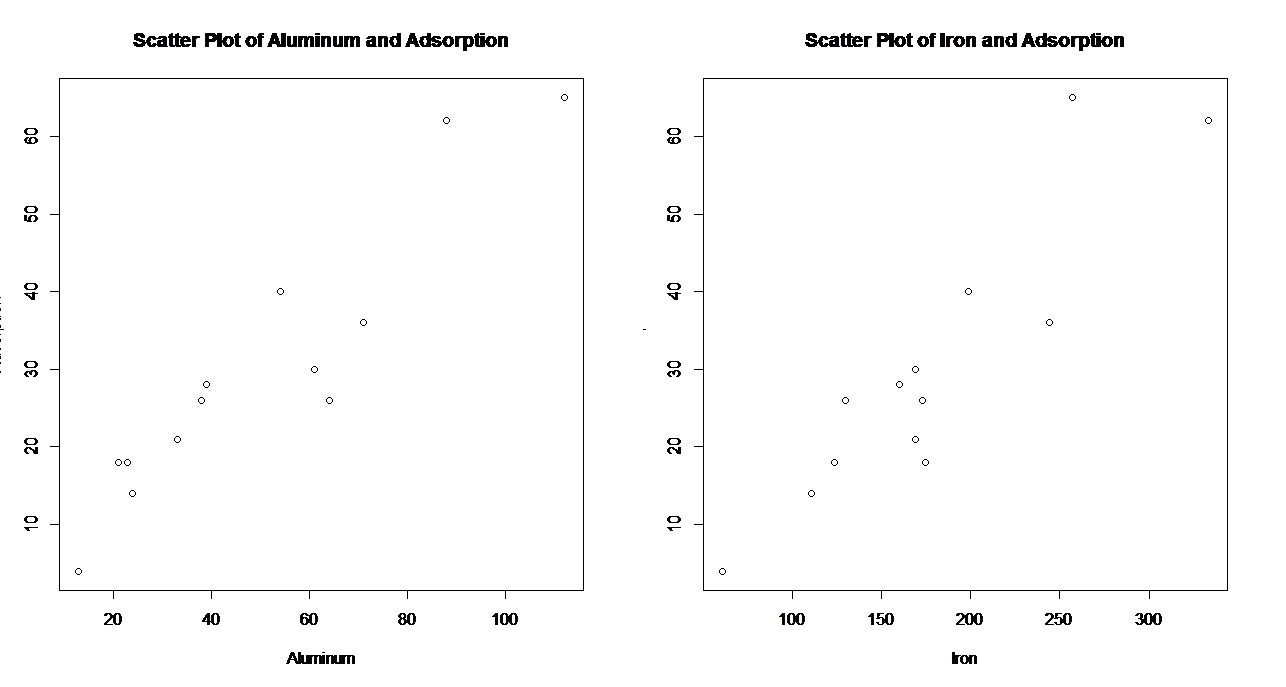
\includegraphics[scale=0.3]{scattermlr}\\
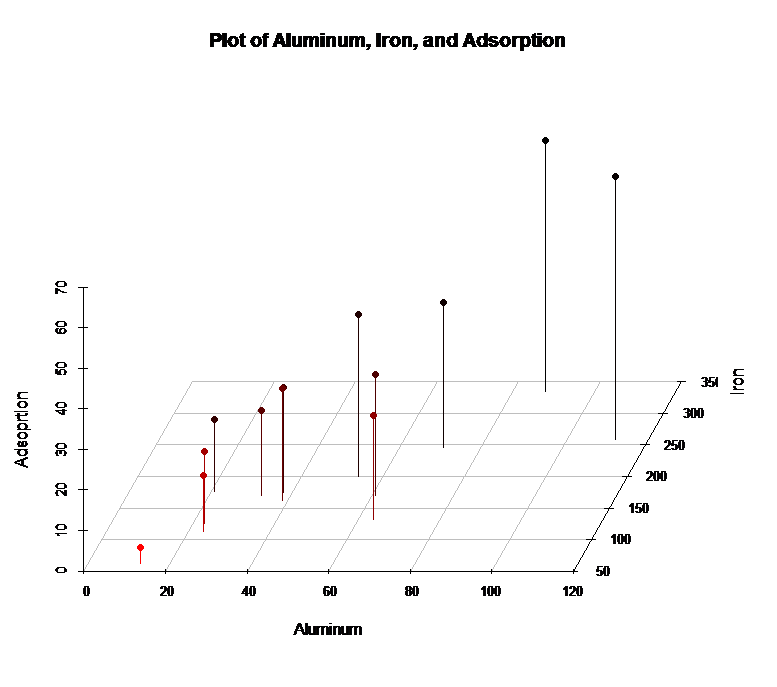
\includegraphics[scale=0.4]{scatter3dmlr}
\end{center}

\newpage

In this case, we don`t want to find the best fitting line, but rather the best fitting \textit{plane} (the one the minimizes the squared distances between the plane and the data points). Our hypothesis of interest is that at least one of our variables is useful (i.e. at least one partial slope is truly non-zero).  We can then test
$$H_0: \beta_1=\beta_2=0 ~~vs~~H_A: \text{ at least one is non-zero}$$


When we fit an MLR model with $p$ different predictors we are really attempting to find the best `response surface' of degree $p$ in a $p+1$ dimensional space.  For instance, with one predictor, we are fitting the best line in a 2-d space.  The plots below give a number of surfaces that can be fit using two predictors when quadratic or interaction terms are included.

\begin{center}
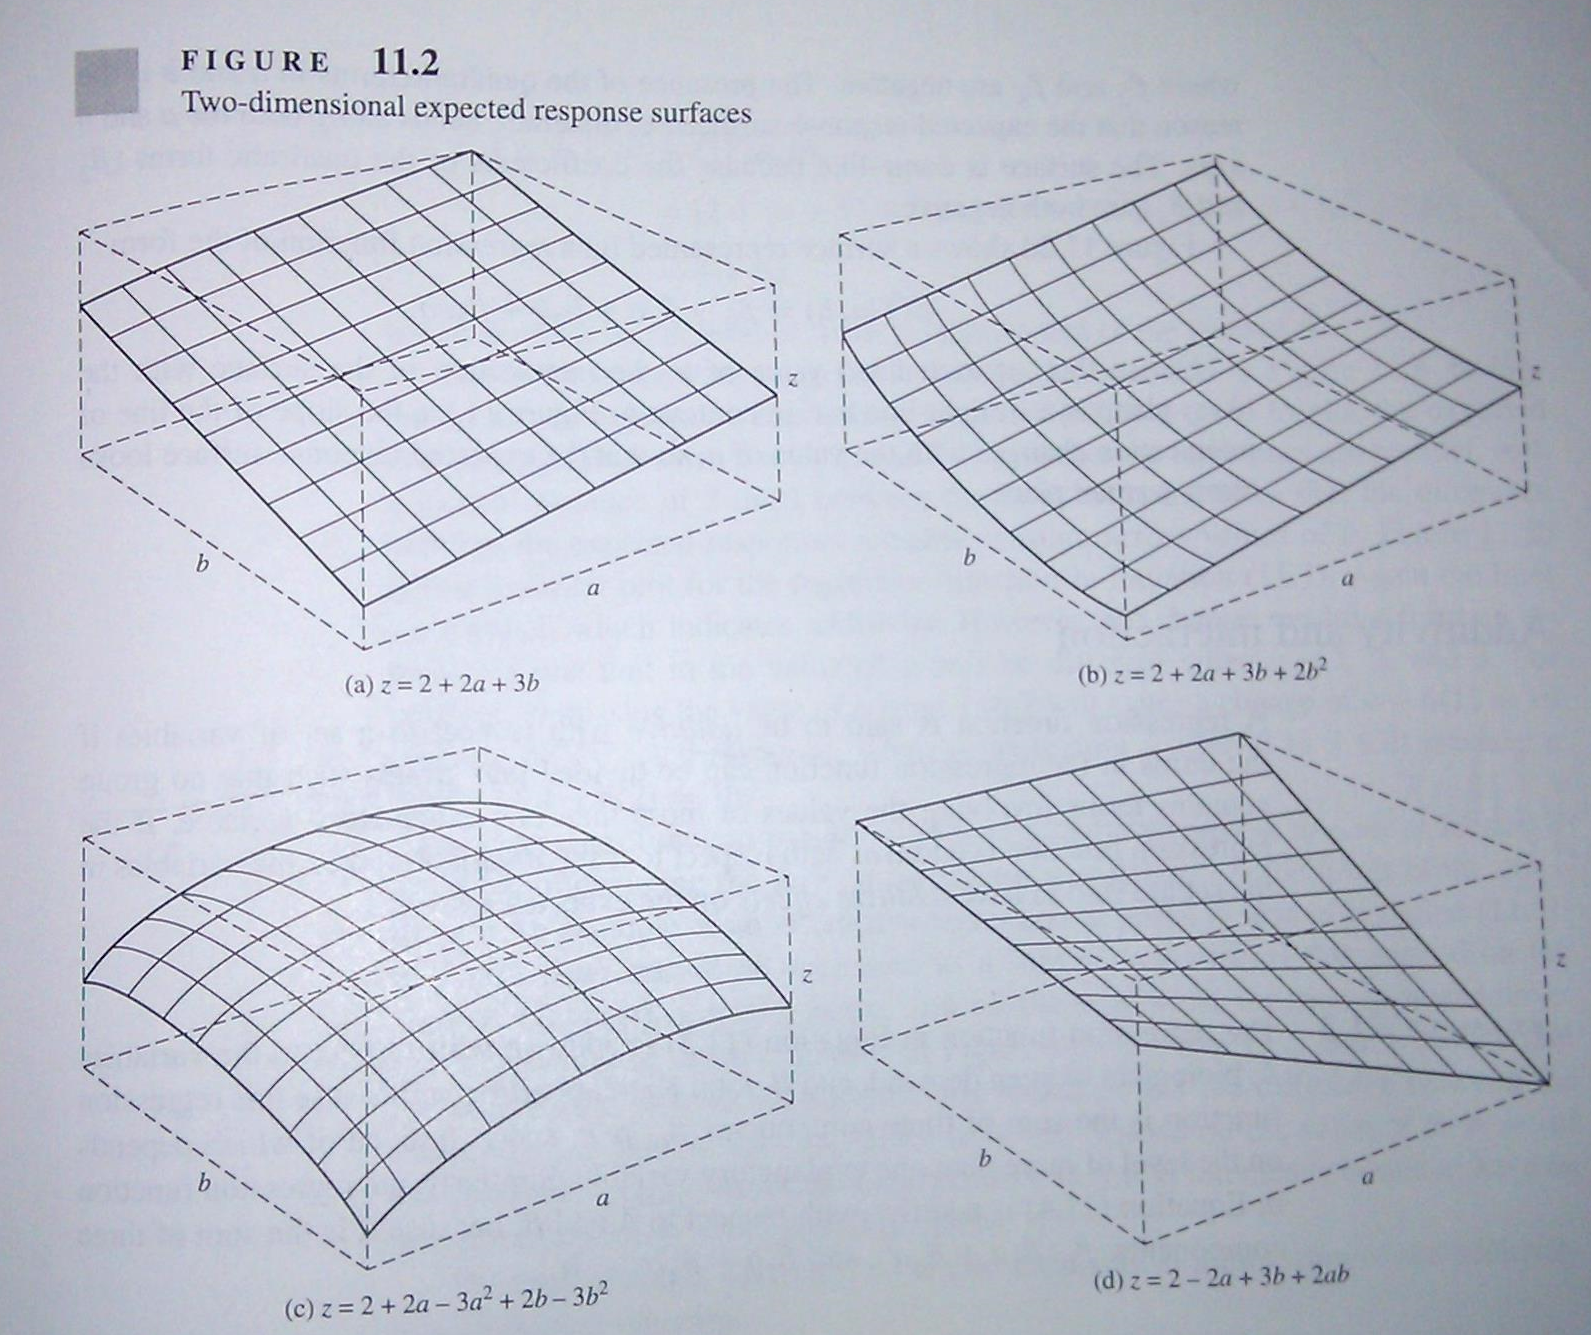
\includegraphics[scale=0.3]{surfaces}
\end{center}

A link to visualizing different surfaces:  \begin{verbatim} http://www.ats.ucla.edu/stat/sas/teach/reg_int/reg_int_cont.htm \end{verbatim}~\\

\newpage

\textbf{Very brief matrix review:}\\
Note: Capital boldface letters are usually used for matrices and boldface lower case letters are usually used for vectors (matrices where the number of rows or the number of columns is 1).\\~\\
\textbf{Matrices} - rectangular arrays of numbers that have a great many uses.  Some matrices, (with {\em dimension} in parentheses):
\[
\begin{array}{cccc}
\textbf{A}&=&\left(\begin{array}{cc} 7 & 5 \\ 5 & 2 \\ 3 & 2 \end{array}\right)  & (3 \times 2) \\
\textbf{B}&=&\left(\begin{array}{ccc} 4 & 2 & 1 \\ 3 & 1 & 1 \end{array}\right)  & (2 \times 3)  \\
\textbf{C}&=&\left(\begin{array}{cc} 1 & 1 \\ -1 & 1 \end{array}\right) & (2 \times 2) \\
\textbf{I}_2&=&\left(\begin{array}{cc} 1 & 0 \\ 0 & 1 \end{array}\right) & (2 \times 2)
\end{array}
\]
\textbf{Matrix operations}
\begin{enumerate}
\item \underline{Transposition} - swap rows for columns, columns for rows:
\[
t(\textbf{A}) = \textbf{A}` =
\left(\begin{array}{ccc} 7 & 5 & 3 \\ 5 & 2 & 2 \end{array}\right) \ \ \mbox{``transpose of $\textbf{A}$"}
\]
\item
Addition is elementwise, matrices must have same {\em dimension}
\[ 
\textbf{C} + \textbf{I}_2 = 
\left(\begin{array}{cc} 1 + 1 & 1 + 0 \\ -1 + 0  & 1 + 1 \end{array}\right) 
=
\left(\begin{array}{cc} 2 & 1 \\ -1 & 2 \end{array}\right) \ \ (2 \times 2)
\]
Subtraction, same deal
\[ 
\textbf{C} - \textbf{I}_2 = \left(\begin{array}{cc} 0 & 1 \\ -1 & 0 \end{array}\right) \ \ (2 \times 2)
\]
\item
Multiplication requires {\em conformability}.  Element in $i^{th}$ row, $j^{th}$ column of $\textbf{AB}$ is dot-product of $i^{th}$ row of $\textbf{A}$, $j^{th}$ column of $\textbf{B}$:
\[ 
\begin{array}{ccc}
\textbf{AB} & = & 
\left(\begin{array}{cc} 7 & 5 \\ 5 & 2 \\ 3 & 2 \end{array}\right)  
\left(\begin{array}{ccc} 4 & 2 & 1 \\ 3 & 1 & 1 \end{array}\right)  
\\
%\]
%\[
\textbf{AB} & = & \left(\begin{array}{ccc} 
7 \cdot 4 + 5 \cdot 3, & 
7 \cdot 2 + 5 \cdot 1, & 
7 \cdot 1 + 5 \cdot 1 \\
5 \cdot 4 + 2 \cdot 3, & 
5 \cdot 2 + 2 \cdot 1, & 
5 \cdot 1 + 2 \cdot 1 \\
3 \cdot 4 + 2 \cdot 3, & 
3 \cdot 2 + 2 \cdot 1, & 
3 \cdot 1 + 2 \cdot 1 \end{array}\right) \\
& = & \left(\begin{array}{ccc} 43 & 19 & 12 \\ 26 & 12 & 7 \\ 18 & 8 & 5 \end{array}\right) \end{array}
\] 

(The product $\textbf{DE}$ is not necessarily equal to $\textbf{ED}$).  The matrices $\textbf{D}$ and $\textbf{E}$ are conformable for the product $\textbf{DE}$ if $\textbf{D}$ has the same number of columns as $\textbf{E}$ has rows.  Note that in the product of $\textbf{AB}$ of the matrices given above, $\textbf{A} (3 \times 2)$ and $\textbf{B} (2 \times 3)$ are conformable.\\~\\

$\textbf{I}$ is reserved for the {\em identity} matrix, which is {\em square},
{\em symmetric}, {\em diagonal} with $1's$ along the diagonal and $0's$
elsewhere:
$$ \textbf{I}_3 = \left(\begin{array}{ccc} 1 & 0 & 0 \\ 0 & 1 & 0 \\ 0 & 0 & 1 \end{array}\right) $$
Multiplication of any (conformable) matrix $\textbf{M}$ by $\textbf{I}$ gives $\textbf{M}$:
$\textbf{AI}_3 = \textbf{A} = \textbf{I}_2 \textbf{A}$
\item Inversion.  The {\em inverse} $\textbf{M}^{-1}$ of a {\em square} ($r \times r$) matrix $\textbf{M}$,
if it exists, satisfies $\textbf{MM}^{-1}=\textbf{I}_r$ (similar to the reciprocal of real number).  A square matrix with an inverse is called
{\em non-singular}.\\
Inversion can be computationally challenging, but not for
$(2 \times 2)$ case:
$$ \left(\begin{array}{cc} a & b \\ c & d \end{array}\right) = 
\frac{1}{ad-bc}
\left(\begin{array}{cc} d & -b \\ -c & a \end{array}\right) $$
Find $\textbf{C}^{-1}$.
$$\textbf{C}^{-1} = \frac{1}{2}\left(\begin{array}{cc} 1 & -1 \\ 1 & 1\end{array}\right)$$

The {\em rank} of a matrix is equal to the number of {\em linearly independent}
rows or columns of the matrix.  Vectors $\textbf{x}_1,\textbf{x}_2,\ldots,\textbf{x}_n$ are linearly independent
if $\sum_i a_i \textbf{x}_i = 0$ implies $a_1=a_2=\cdots=a_n=0$.

Matrix uses: model statements, systems of linear equations, covariance matrices of random vectors,\ldots.

Consider two lines $y_1=5-x, y_2=3+x$.  Do these lines intersect?  Where?
Write this system of two equations in two unknowns using a matrix:
$$ \textbf{C} \left(\begin{array}{c} x \\ y\end{array}\right) = \left(\begin{array}{c} 5 \\ 3\end{array}\right)$$
(left-multiply both sides by $\textbf{C}^{-1}$) 
$$ \left(\begin{array}{c} x \\ y\end{array}\right) = \textbf{C}^{-1} \left(\begin{array}{c} 5 \\ 3\end{array}\right) = \left(\begin{array}{c}1 \\ 4 \end{array}\right)$$
The lines intersect at the solution, $(x=1,y=4)$.
\end{enumerate}

Matrices are cool and very useful!\\~\\

If we have a random vector (just like a random variable but in vector form, i.e. components yield numeric answers that are random), call it $\textbf{Y}$, and a constant vector, call it \textbf{a}, then
$$E(\textbf{a}'\textbf{Y}) = \textbf{a}'E(\textbf{Y})$$
$$\Var(\textbf{a}'\textbf{Y}) = \textbf{a}'\Var(\textbf{Y})\textbf{a}$$

Understanding matrices if very important as this is how we will look at our models for much of the rest of the class.  Also, SAS and other statistical programs use matrices in their calculations and in their output.

\newpage

\textbf{Matrix formulation of MLR}\\
\begin{center}
$\textbf{Y} = \textbf{X}\boldsymbol{\beta} + \textbf{E}$
\end{center}
All of the response RVs are placed into the \textbf{response vector}:
$$\textbf{Y}=\left(\begin{array}{c}
Y_1\\
Y_2\\
\vdots\\
Y_n\\
\end{array}\right)$$
For observation $i$ we can group all of the explanatory variables into a vector
$$\textbf{x}_{i} = (1,x_{i1},x_{i2},x_{i3},\ldots,x_{ip}).$$
The 1 in the first spot of the vector is for the intercept.  If we `stack' these row vectors on top of each other we can make a matrix called the \textbf{design matrix}:
$$
\textbf{X}=\left(\begin{array}{ccccc}
1  &  x_{11}  &   x_{12} & \ldots & x_{1p} \\
1  &  x_{21}  &   x_{22} & \ldots & x_{2p} \\
\vdots &\vdots &\vdots &\vdots &\vdots \\ 
1  &  x_{n1}  &   x_{n2} & \ldots & x_{np} \\
\end{array}\right)$$

We also form a column vector corresponding to the regression parameters, called the \textbf{`beta vector'}:
$$\boldsymbol{\beta}=\left(\begin{array}{c}
\beta_0\\
\beta_1\\
\vdots\\
\beta_p\\
\end{array}\right)$$

and a column vector for the error terms, called the \textbf{error vector}:
$$\textbf{E}=\left(\begin{array}{c}
E_0\\
E_1\\
\vdots\\
E_n\\
\end{array}\right)$$


Now we can see that our MLR model (a system of $n$ equations with $p+1$ unknowns) 
\begin{eqnarray*}
Y_1 & = & \beta_0 + \beta_1 x_{11} + \beta_2 x_{12}+ \cdots + \beta_p x_{1p} + E_1 \\
Y_2 & = & \beta_0 + \beta_1 x_{21} + \beta_2 x_{22}+ \cdots + \beta_p x_{2p} + E_2 \\
\vdots & = & \vdots \\
Y_n & = & \beta_0 + \beta_1 x_{n1} + \beta_2 x_{n2}+ \cdots + \beta_p x_{np} + E_n
\end{eqnarray*}
can be easily rewritten as
\begin{center}
$\textbf{Y} = \textbf{X}\boldsymbol{\beta} + \textbf{E}$
\end{center}

Our assumptions on the errors can now be specified as $\textbf{E}\sim N_n(\boldsymbol{0},\sigma^2 \textbf{I}_{n})$ (multivariate normal distribution).  $\sigma^2 \textbf{I}_{n}$ is called the variance-covariance matrix:
$$
Var(\textbf{E})=\left(\begin{array}{cccc}
\sigma^2  &  0  &   \ldots & 0 \\
0  &  \sigma^2  &   \ldots & 0 \\
\vdots &\vdots &\vdots &\vdots  \\ 
0  &  0  &  \ldots & \sigma^2 \\
\end{array}\right)$$

The diagonals of the matrix give the variances for the $E_i$`s ($Var(E_1), Var(E_2), \ldots, Var(E_n)$) and the off-diagonals (say row $i$ column $j$) give the covariances between $E_i$`s and the $E_j$`s ($Cov(E_i, E_j)$).  As the off-diagonals are all 0, our errors are uncorrelated (which for the multivariate normal distribution implies independence).\\~\\

Let`s look at some of these quantities for our adsorption example.  We have $n=13$ and $p=2$.
\begin{center}
\begin{tabular}{ccc}
\textbf{y}=$\left(\begin{array}{c} 4 \\18\\14\\18\\26\\26\\21\\30\\28\\36\\65\\62\\40\\\end{array}\right)$ &
\textbf{X}=$\left(\begin{array}{ccc}1&13& 61\\1&21&175\\1&24&111\\1&23&124\\1&64&130\\1&38&173\\1&33&169\\1&61&169\\1&39&160\\1&71&244\\1&112&257\\1&88&333\\1&54&199\\\end{array}\right)$&
$\boldsymbol{\beta}$=$\left(\begin{array}{c} \beta_0 \\\beta_1\\\beta_2\\\end{array}\right)$ 
\end{tabular}
\end{center}

\newpage

The predicted values can be written as
$$\hat{\textbf{y}} = \textbf{X} \hat{\boldsymbol{\beta}} = \textbf{X} (\textbf{X}'\textbf{X})^{-1} \textbf{X}'\textbf{y} = \textbf{H} \textbf{y} $$
and residuals as
$$\textbf{e}  =  \textbf{y}-\hat{\textbf{y}}  =  \textbf{y} - \textbf{X}\hat{\boldsymbol{\beta}} =  (\textbf{I}-\textbf{H}) \textbf{y}$$

\begin{itemize}
\item $\hat{\textbf{y}}$ is called the vector of \underline{fitted} or \underline{predicted values}
\item $\textbf{H}=\textbf{X}(\textbf{X}'\textbf{X})^{-1}\textbf{X}$ is called the \underline{hat matrix} as it `places' the hat on $\textbf{y}$
\item $\textbf{e}$ is the vector of \underline{residuals}
\end{itemize}

We will still use least squares to select the parameters, which can be written as the minimum of:
$$SS(E) = \sum_{i=1}^{n}(obs_i-pred_i)^2=\sum_{i=1}^n(y_i-\hat{y}_i)^2=\sum_{i=1}^n (y_i - \beta_0 - \beta_1 x_{i1} - \cdots - \beta_p x_{ip})^2=\textbf{e}'\textbf{e}$$

For the adsorption example, many of these matrices are given below:
\begin{center}
\begin{tabular}{cc}
\textbf{X}'\textbf{X} = $\left(\begin{array}{ccc} 13&641&2305\\ 641&41831 & 133162\\ 2305&133162 &467669\\\end{array}\right)$ &
$(\textbf{X}'\textbf{X})^{-1}$ = $\left(\begin{array}{ccc} 0.633138 &0.002477&-0.003826\\ 0.002477 & 0.000265 & -0.000088\\ -0.003826 &-0.000088 &0.000046 \\\end{array}\right)$ 
\end{tabular}
\end{center}

\begin{center}
\begin{tabular}{cc}
$\hat{\boldsymbol{\beta}}= (\textbf{X}'\textbf{X})^{-1} \textbf{X}'\textbf{Y}$ = $\left(\begin{array}{cc} -7.3507\\  0.3490\\ 0.1127\\\end{array}\right)$&
$\hat{\textbf{y}} = \textbf{X}\hat{\boldsymbol{\beta}} = \left(\begin{array}{c}4.0610\\19.7008\\13.5350\\14.6511\\29.6363\\25.4084\\23.2126\\32.9846\\24.2923\\44.9271\\60.7012\\60.8904\\33.9226\\\end{array}\right)$
\end{tabular}
\end{center}

$$SS(E) = \textbf{e}'\textbf{e} = 191.7897 ~~~~~ \hat{\sigma}^2=MS(E) = SS(E)/(n-p-1) = 191.7897/10 = 19.17897 $$

$$\hat{\boldsymbol{\Sigma}}=MS(E)(\textbf{X}'\textbf{X})^{-1} = \left(\begin{array}{ccc}
 12.14294&  0.04750& -0.07337\\
 0.04750  &0.00508 &-0.00168\\
 -0.07337 &-0.00168&  0.00088\\
\end{array}\right)$$

\newpage

The parameter estimates and the variance-covariance matrix are very useful for making inference about our intercept and partial slope parameters (done very similary to SLR).  Let`s use the above to find the following
\begin{enumerate}
\item What is the estimate for $\beta_2$?  What is the interpretation?
\item What is the standard error of $\hat\beta_2$?  
\item Conduct a test to determine if $\beta_2=0$ plausible (technically, after accounting for the linear association between extractable aluminum and adsorption index).  Hint: $t(0.025, 10)=2.228$
\item Estimate the mean adsorption index among the population of ALL soil with extractable aluminum = 100 and extractable iron = 150.  Report a standard error for this estimate and a $95\%$ confidence interval and a 95\% prediction interval.
\end{enumerate}

\newpage

Recall that the overall hypotheses we want to test are
$$H_0: \beta_1=\beta_2=0 ~~vs~~H_A: \text{ at least one is non-zero}$$
This is the test done in the ANOVA table given in the output from a MLR model.  This is called the \textbf{global $F$-test} as it tests whether at least one of the terms in the model is important for predicting the response.\\~\\

The ANOVA table for MLR follows the same ideas as in SLR.  We are taking the total amount of variation in the response (SS(Tot)) and partitioning it into a part due to the model (SS(R)) and a part due to experimental error (SS(E)).  In fact, the formulas for the sums of squares remain the same, only the degrees of freedom and the $F$-distribution used for finding the p-value change.\\~\\

The full ANOVA table for MLR is given below:\\
\begin{tabular}{|c|c|c|c|c|} \hline
Source & Sum of squares & df & Mean Square & F-Ratio \\ \hline
Regression & $SS(R)$ & p & $MS(R)$ & $MS(R)/MS(E)$ \\
Error & $SS(E)$ & $n-p-1$ & $MS(E)$ &  \\
Total & $SS(Tot)$ & $n-1$ & &  \\ \hline
\end{tabular}
~\\~\\
\textbf{How to do MLR in SAS?}\\~\\
The following code will produce output appropriate for analysis:
\begin{small}
\begin{verbatim}
proc reg data=adexp ;
model adsorp=aluminum iron/clb;
run;
\end{verbatim}
\end{small}

\begin{center}
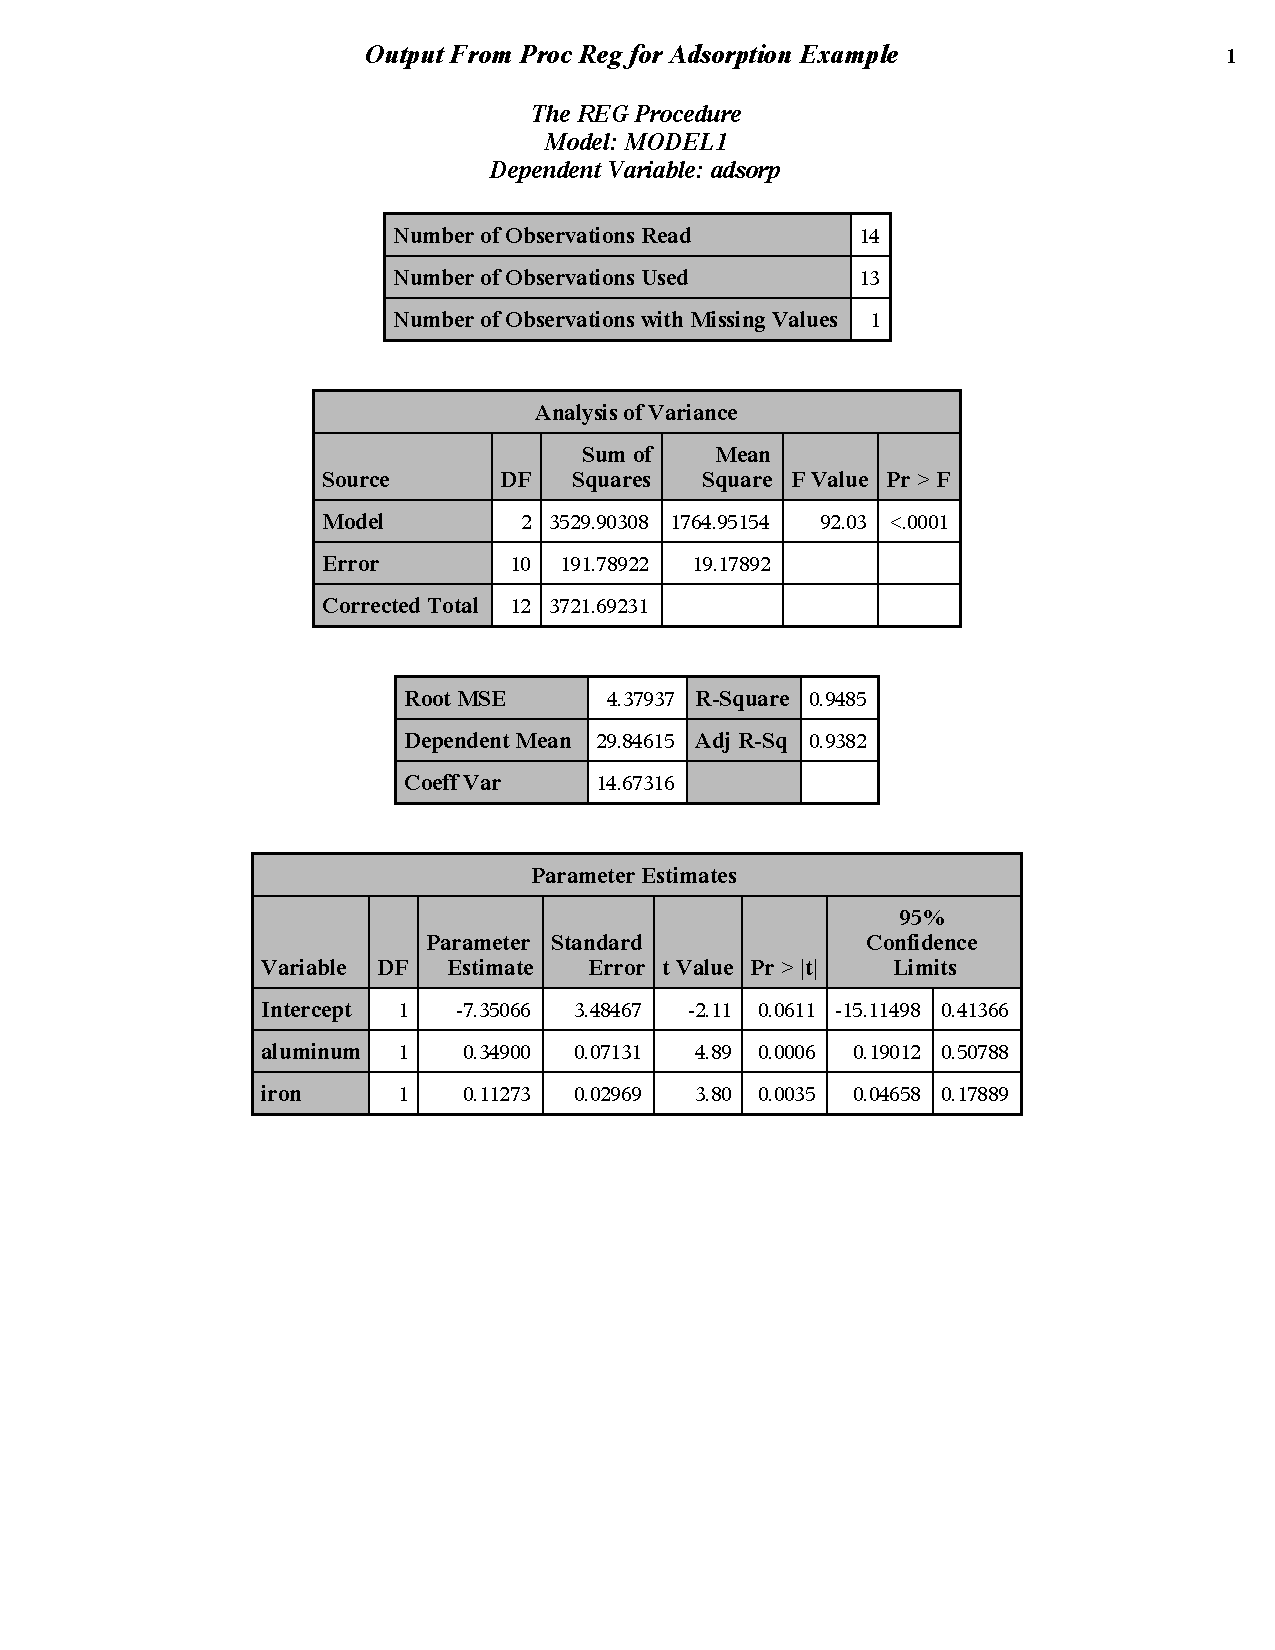
\includegraphics[page=1,scale=0.55,trim = 20mm 70mm 20mm 20mm]{mlradexp}\\
\end{center}

\begin{center}
\includegraphics[page=2,scale=0.55,trim = 20mm 60mm 20mm 20mm]{mlradexp}\\
\includegraphics[page=3,scale=0.4,trim = 20mm 120mm 20mm 20mm]{mlradexp}
\end{center}

\newpage

\textbf{A non-additive model example:}\\
A random sample of students taking the same exam:
\begin{center}
\begin{tabular}{|c|c|c|} \hline
IQ & Study TIME & GRADE \\ \hline
105 & 10 & 75 \\
110 & 12 & 79 \\
120 & 6 & 68 \\
116 & 13 & 85 \\
122 & 16 & 91 \\
130 & 8 & 79 \\
114 & 20 & 98 \\
102 & 15 & 76 \\ \hline
\end{tabular}
\end{center}

Consider regressing GRADE on IQ ($X_1$), TIME($X_2$), and TI ($X_1*X_2$), where TI = TIME*IQ.  That is, we fit the model:
$$Y=\beta_0+\beta_1X_1 +\beta_2X_2+\beta_3X_1X_2+E$$
\begin{small}
\begin{verbatim}
proc reg;
model Grade = IQ Time TI;
run;

                                      The SAS System                                     1
                                    The REG Procedure

                                   Analysis of Variance
 
                                          Sum of           Mean
      Source                   DF        Squares         Square    F Value    Pr > F

      Model                     3      610.81033      203.60344      26.22    0.0043
      Error                     4       31.06467        7.76617                   
      Corrected Total           7      641.87500                                    

                                   Parameter Estimates
 
                    Parameter     Standard
   Variable   DF     Estimate        Error  t Value  Pr > |t|
   Intercept   1     72.20608     54.07278     1.34    0.2527
   IQ          1     -0.13117      0.45530    -0.29    0.7876
   Time        1     -4.11107      4.52430    -0.91    0.4149
   TI          1      0.05307      0.03858     1.38    0.2410 
\end{verbatim}
\end{small}

\newpage

Discussion of the interaction model:\\
 We call the product TI = Time*IQ an "interaction" term. That is, our explanatory variables do not have an independent effect on the response.
$$ \widehat{Mean Grade} = 72.21 - 0.13*IQ - 4.11*Time + 0.0531*TI$$ 
Now if IQ = 100 we get
$$ \widehat{Mean Grade} = (72.21 - 13.1) + (- 4.11 + 5.31)*Time$$
and if IQ  120 we get
$$ \widehat{Mean Grade} = (72.21 - 15.7) + (- 4.11 + 6.37)*Time.$$
Thus we expect an extra hour of study to increase the grade by 1.20 points for someone with IQ = 100 and by 2.26 points for someone with IQ = 120 if we use this interaction model.\\~\\
Generally, we can interpret the (true) $\beta$ parameters in the model as:
\begin{itemize}
\item $\beta_0$ - Average value of Grade when IQ and Study Time are 0
\item $\beta_1$ - Average change in Grade for a unit increase in IQ when Study Time is 0
\item $\beta_2$ - Average change in Grade for a unit increase in Study Time when IQ is 0
\item $\beta_3$ - Average change in the slope for IQ (or Study Time) for a given value of Study Time (or IQ).
\end{itemize}
The interpretation of the interaction `slope' can be seen by looking at the following:
$$\mu(x_1+1,x_2)-\mu(x_1,x_2)=\beta_0+\beta_1(x_1+1)+\beta_2x_2+\beta_3(x_1+1)(x_2)-\beta_0-\beta_1x_1-\beta_2x_2-\beta_3x_1(x_2)$$
$$=\beta_1+\beta_3x_2$$
So $\beta_3$ is the amount the slope for $x_1$ changes per unit change in $x_1$ while $x_2$ is held constant.\\~\\

Note:  The global p-value is significant, but none of our individual terms are.   This gives evidence that our model is over-fit.  we may want to go back to the simpler ``main effects'' model.  \\~\\

\newpage

\textbf{Model Selection:}\\

$x_1,x_2,x_3$ denote $p$ independent variables.  Consider
several models:
\begin{enumerate}
\item $\mu(x_1,x_2,x_3) = E(Y|x_1,x_2,x_3) =  \beta_0 + \beta_1 x_1$
\item $\mu(x_1,x_2,x_3) = E(Y|x_1,x_2,x_3) =  \beta_0 + \beta_2 x_2$
\item $\mu(x_1,x_2,x_3) = E(Y|x_1,x_2,x_3) =  \beta_0 + \beta_3 x_3$
\item $\mu(x_1,x_2,x_3) = E(Y|x_1,x_2,x_3) =  \beta_0 + \beta_1 x_1 + \beta_2 x_2 + \beta_3 x_3$
\item $\mu(x_1,x_2,x_3) = E(Y|x_1,x_2,x_3) =  \beta_0 + \beta_1 x_1 + \beta_3 x_3$
\item $\mu(x_1,x_2,x_3) = E(Y|x_1,x_2,x_3) =  \beta_0 + \beta_1 x_1 + \beta_2 x_2$
\item $\mu(x_1,x_2,x_3) = E(Y|x_1,x_2,x_3) =  \beta_0 + \beta_2 x_2 + \beta_3 x_3$
\end{enumerate}
$A$ is nested in $B$ means model $A$ can be obtained by restricting (e.g. setting to 0) parameter values in model $B$.

\textbf{True or false:}
\begin{itemize}
\item Model 1 nested in Model 4 ~~~~~~~~~~~~~~~~~Model 1 nested in Model 5
\item Model 2 nested in Model 4 ~~~~~~~~~~~~~~~~~Model 4 nested in Model 1
\item Model 3 nested in Model 4 ~~~~~~~~~~~~~~~~~Model 5 nested in Model 4
\item Model 3 nested in Model 7 ~~~~~~~~~~~~~~~~~Model 1 nested in Model 7
\end{itemize}

$A$ nested in $B$ $\longrightarrow$ $A$ called {\em reduced model}, $B$ called {\em full model}.  \\~\\

$p$ - number of regression parameters in full model  \\
$q$ - number of regression parameters in reduced model \\
$p-q$ - number of regression parameters being tested. \\~\\

Let`s get a handle on this notation.  Give the extra regression $SS$ terms for comparing some of the nested models on preceding page:
\begin{itemize}
\item Model 1 in model 4: $R(\beta_2,\beta_3|\beta_1)$
\item Model 2 in model 4:  
\item Model 3 in model 4:  
\item Model 1 in model 5: $R(\beta_3|\beta_1) $
\item Model 5 in model 4:
\end{itemize}


\textbf{An example: How to measure body fat?} \\
For each of $n=20$ healthy individuals, the following measurements were made: bodyfat percentage $y_i$, triceps skinfold thickness, $x_{1}$, thigh circumference $x_{2}$, midarm circumference $x_{3}$.\\

\begin{small}
\begin{verbatim}
  x1    x2    x3    y
  19.5  43.1  29.1  11.9
  24.7  49.8  28.2  22.8                   ods graphics on;
  30.7  51.9  37.0  18.7                   proc corr plots=matrix;
  29.8  54.3  31.1  20.1                   var y x1 x2 x3;
  19.1  42.2  30.9  12.9                   run;
  25.6  53.9  23.7  21.7
  31.4  58.5  27.6  27.1
  27.9  52.1  30.6  25.4
  22.1  49.9  23.2  21.3
  25.5  53.5  24.8  19.3
  31.1  56.6  30.0  25.4
  30.4  56.7  28.3  27.2
  18.7  46.5  23.0  11.7
  19.7  44.2  28.6  17.8
  14.6  42.7  21.3  12.8
  29.5  54.4  30.1  23.9
  27.7  55.3  25.7  22.6
  30.2  58.6  24.6  25.4
  22.7  48.2  27.1  14.8
  25.2  51.0  27.5  21.1
\end{verbatim}
\end{small}

\begin{center}
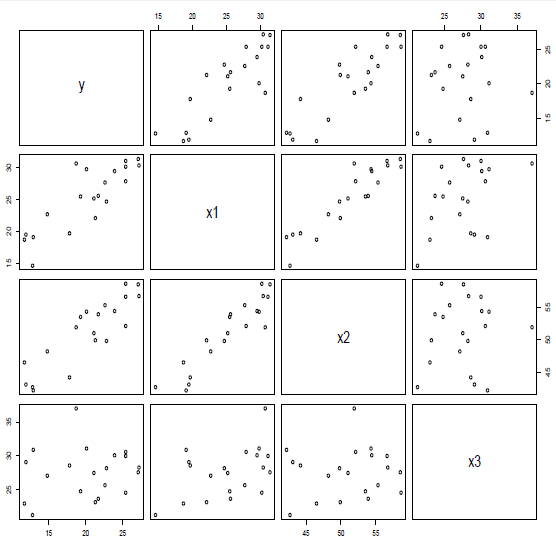
\includegraphics[height=3.7in,width=3.7in]{bodyfat}
\end{center}

\newpage

\begin{small}
\begin{verbatim}
                Pearson Correlation Coefficients, N = 20 
                        Prob > |r| under H0: Rho=0
 
                       y            x1            x2            x3

        y        1.00000       0.84327       0.87809       0.14244
                                <.0001        <.0001        0.5491

        x1       0.84327       1.00000       0.92384       0.45778
                  <.0001                      <.0001        0.0424

        x2       0.87809       0.92384       1.00000       0.08467
                  <.0001        <.0001                      0.7227

        x3       0.14244       0.45778       0.08467       1.00000
                  0.5491        0.0424        0.7227              
\end{verbatim}
\end{small}

Looking at the scatter plots and the correlation output, marginal associations between $y$ and $x_1$ and between
$y$ and $x_2$ are highly significant, providing evidence of a strong $r\approx 0.85$ linear association between average
bodyfat and triceps skinfold and between average bodyfat and thigh circumference.\\~\\

Notice the scatter plot between $x_1$ and $x_2$, there is a strong linear relationship.  This means that triceps skinfold and thigh circumference are giving some of the same information.  This can lead to issues when fitting a model.\\~\\
\textbf{Multicollinearity:} linear associations among the independent variables; causes problems such as inflated sampling variances for $\hat{\boldsymbol{\beta}}$.

\begin{small}
\begin{verbatim}
proc reg data=bodyfat;
   model y=x1/covb;
   model y=x2/covb;
   model y=x3/covb;
   model y=x1 x2/covb;
   model y=x1 x2 x3/covb;
run;
\end{verbatim}
\end{small}
Yields the following output:
\begin{center}
\begin{tabular}{cc}
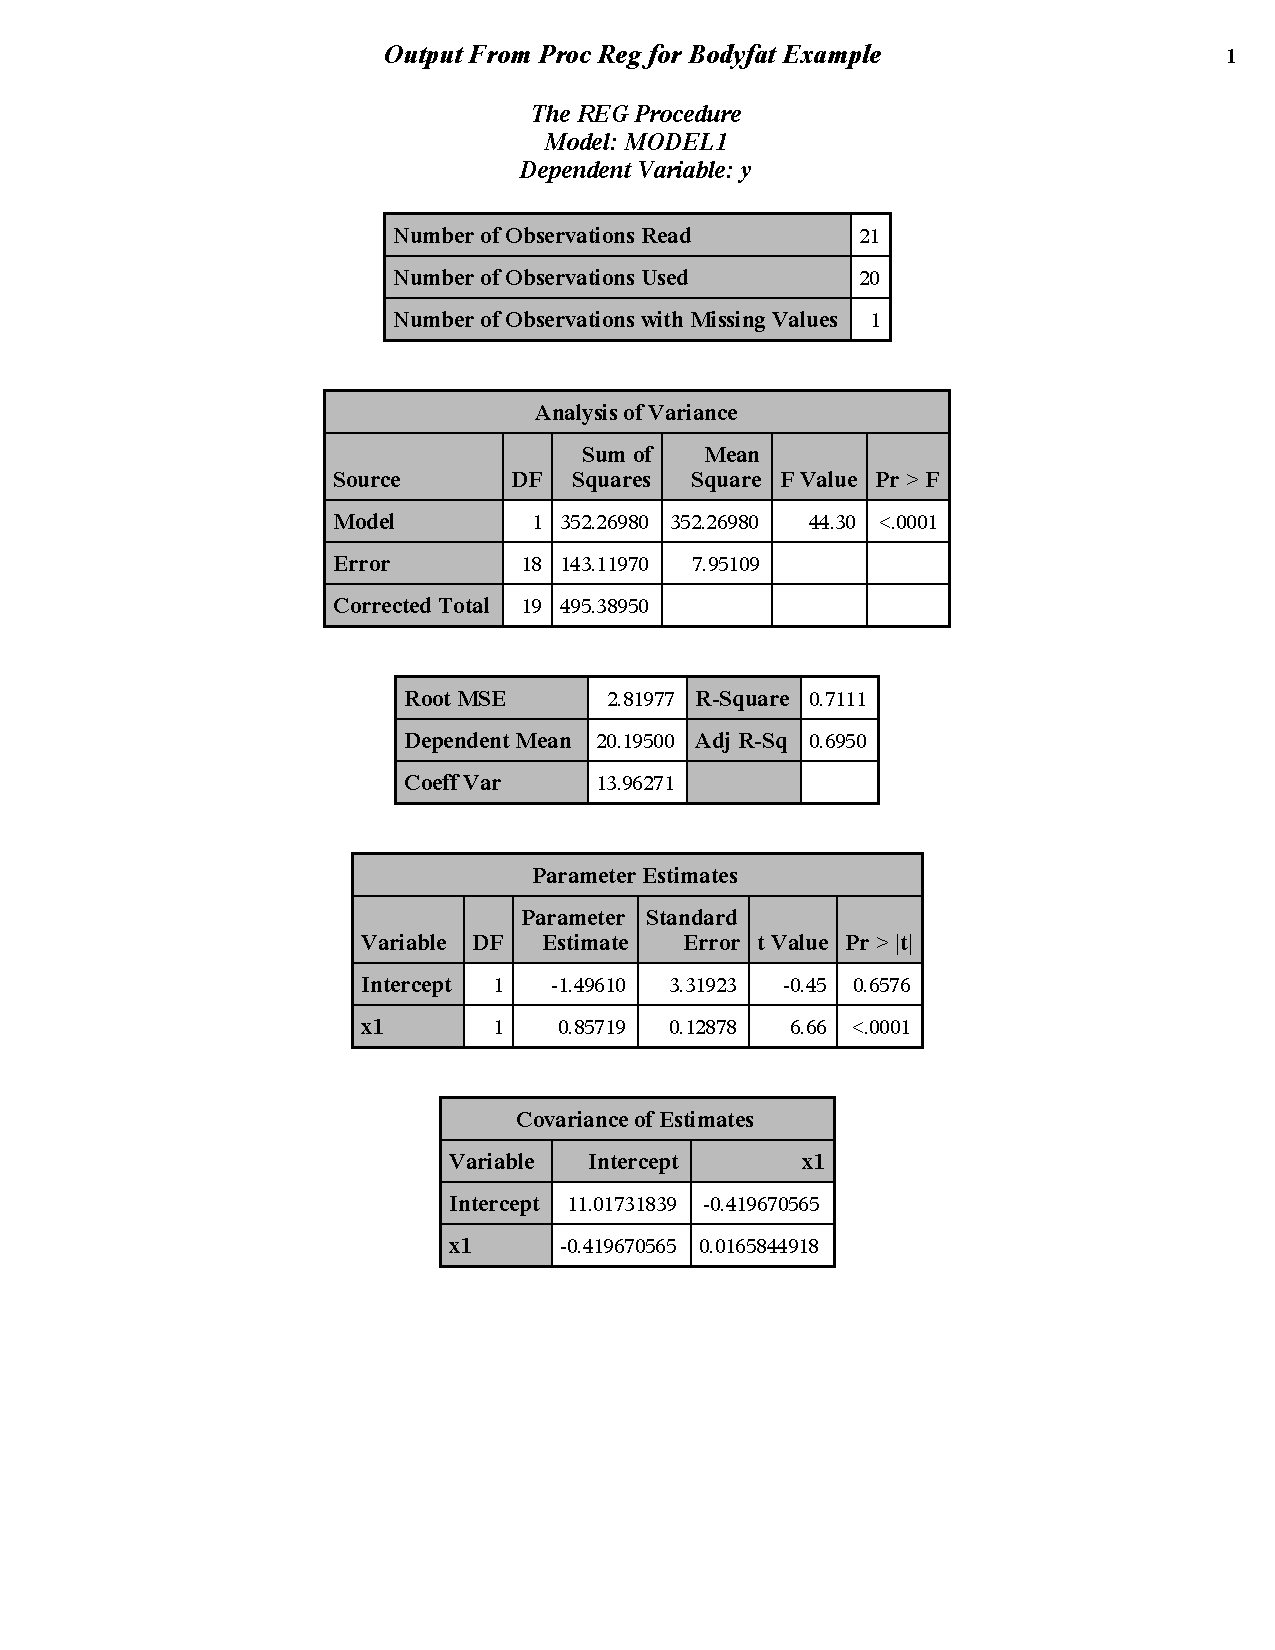
\includegraphics[page=1,scale=0.6,trim=40mm 30mm 20mm 10mm]{bodyfatexample}&
\includegraphics[page=2,scale=0.6,trim=40mm 30mm 20mm 10mm]{bodyfatexample}\\
\end{tabular}
\begin{tabular}{cc}
\includegraphics[page=3,scale=0.6,trim=40mm 30mm 20mm 10mm]{bodyfatexample}&
\includegraphics[page=4,scale=0.6,trim=40mm 30mm 20mm 10mm]{bodyfatexample}\\
\end{tabular}
\includegraphics[page=5,scale=0.6,trim=40mm 30mm 20mm 10mm]{bodyfatexample}
\end{center}

Question:  Why is the global p-value in the last model significant, i.e. at least one predictor is useful, but the individual tests are all nonsignificant?

\newpage

In the bodyfat data, consider comparing the simple model that $Y$ depends only on $x_1$ (triceps) versus the full model that it depends on all three.
\begin{eqnarray*}
\mbox{Model } A: \mu(x_1,x_2,x_3) & = & \beta_0 + \beta_1 x_1 \\
\mbox{Model } B: \mu(x_1,x_2,x_3) & = & \beta_0 + \beta_1 x_1 + \beta_2 x_2 + \beta_3 x_3 
\end{eqnarray*} 
or the null hypothesis 
$$H_0: \beta_2=\beta_3=0 \ \ \mbox{  vs  } \ \ H_1: \beta_2, \beta_3 \mbox{ not both }0$$ 
after accounting for $x_1$.
Our $F$ statistic can be used
$$ F = \frac{(396.9-352.3)/2}{6.15} = \frac{22.3}{6.15}=3.64$$
How many $df$ for numerator and denominator? \\~\\
The $95^{th}$ percentile is $F(0.05,~~~~~~~~ ,~~~~~~~~ ) = 3.63$.\\~\\
Our conclusion about the hypotheses?\\~\\~\\

That is, after accounting for the linear dependence between triceps and bodyfat, there is still some linear association between mean bodyfat and at least one of $x_2,x_3$ (thigh,midarm).  \\~\\

\textbf{To get the nested model $F$-ratio in SAS:}
\begin{small}
\begin{verbatim}
proc reg data=bodyfat;
     model y=x1 x2 x3;
     test x2=0,x3=0;
run;
\end{verbatim}
\end{small}

\begin{center}
\includegraphics[page=4,scale=0.6,trim= 10mm 200mm 10mm 10mm]{bodyfatexampletriceps}
\end{center}

However, we saw in the previous output that a model with all three variables is no good.  This is due to the multicollinearity.  We will now very briefly look at a few automated model selection techniques.

\newpage

\textbf{Using proc reg to perform variable selection:}\\
We`ll discuss three hypothesis testing methods for selecting variables (there are many other ways to accomplish this we won`t discuss).
\begin{enumerate}
\item \textbf{Forward Selection} - Start with nothing and work forward.
	\begin{enumerate}
		\item Begin with a model with only $\beta_0$
		\item Calculate $R(\beta_i|\beta_0)$ for all possible predictors and find p-values for each
		\item Take most significant p-value less than a cutoff (say 0.3), add predictor into model.  
		\item Say $\beta_j$ was added in the last step, repeat above process with added predictor.  That is, calculate $R(\beta_i|\beta_0,\beta_j)$ for all other predictors, etc.
		\item Stop when no predictors are below the cutoff or if the full model is selected.
	\end{enumerate}
\item \textbf{Backward Selection} - Start with everything and work backward. 
\begin{enumerate}
		\item Start with full model.
		\item Locate variable with largest p-value greater than a cutoff (say 0.1), remove that variable.
		\item Repeat until all p-values are less than the cut off or the null model (intercept only model) is chosen.
	\end{enumerate}
\item \textbf{Subset Selection} - Compute all possible models, pick best.
\begin{enumerate}
		\item Compare each of the models using a criterion.
		\item Choose model that minimizes that criterion.  Possible criteria include:
		\begin{itemize}
			\item $Adjusted~R^2 = 1-\frac{n-1}{n-p-1}(1-R^2)$ (takes into account the addition of more predictors)
			\item Mallow`s $C_P$, AIC, AICc, or BIC (all take into account the model complexity, not just how well the model fits the data)
		\end{itemize}
	\end{enumerate}
\end{enumerate}

\textbf{How to do these model selection methods in SAS?}\\
\begin{small}
\begin{verbatim}
proc reg data=bodyfat plots=none;
    model y=x1 x2 x3/selection=cp ;
    model y=x1 x2 x3/selection=forward SLentry=0.3;
    model y=x1 x2 x3/selection=backward SLstay=0.1;
  	model y=x1 x2 x3/selection=adjrsq;
run;
\end{verbatim}
\end{small}

\begin{center}
\begin{tabular}{cc}
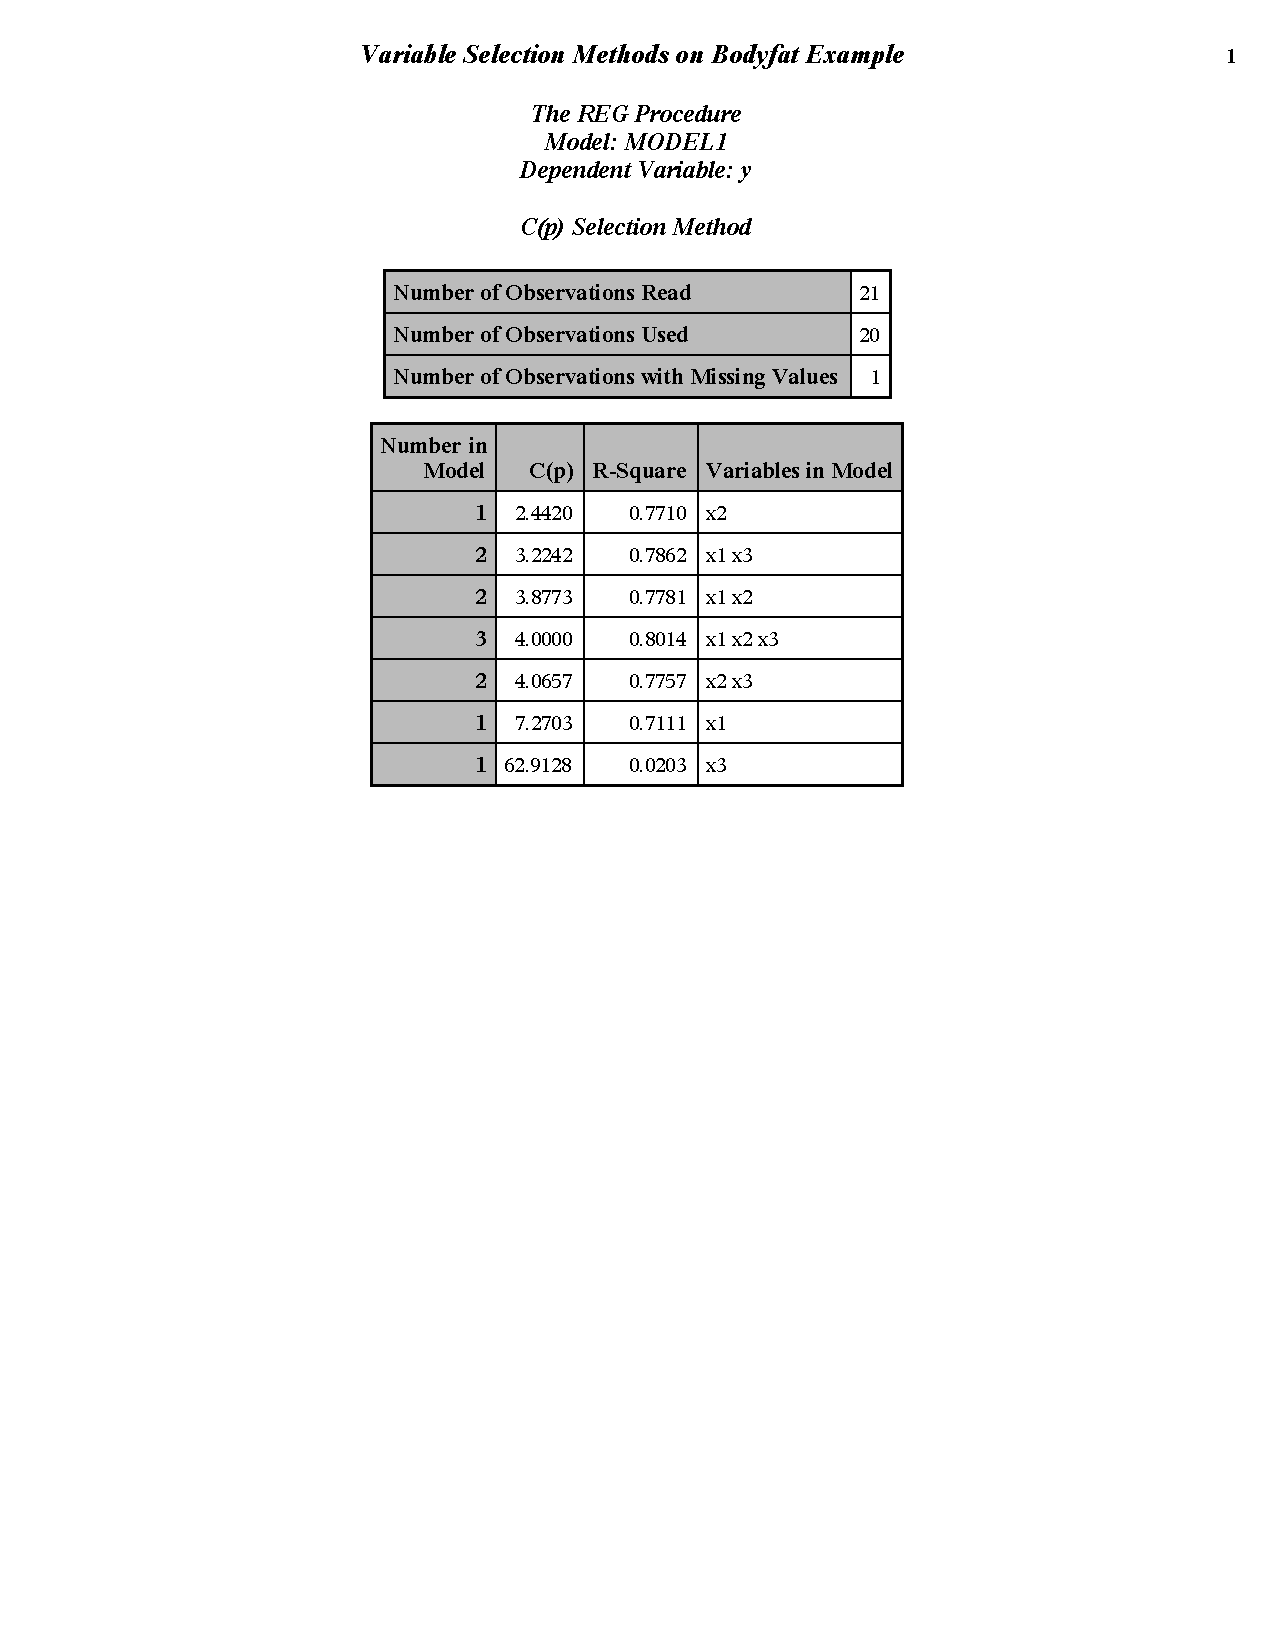
\includegraphics[page=1,scale=0.6,trim=40mm 30mm 20mm 10mm]{bodyfatexampleselection}&
\includegraphics[page=2,scale=0.6,trim=40mm 30mm 20mm 10mm]{bodyfatexampleselection}\\
\end{tabular}
\begin{tabular}{cc}
\includegraphics[page=3,scale=0.6,trim=40mm 30mm 20mm 10mm]{bodyfatexampleselection}&
\includegraphics[page=4,scale=0.6,trim=40mm 30mm 20mm 10mm]{bodyfatexampleselection}\\
\end{tabular}
\includegraphics[page=5,scale=0.6,trim=40mm 120mm 80mm 10mm]{bodyfatexampleselection}
\end{center}

\textbf{Types of Sums of Squares}\\
Given that we have 4 predictors, $X_1-X_4$ we really can have a number of tests based on nested models for $\beta_4=0$ (or for any other $\beta$ for that matter).  Let`s write them down in terms of extra regression sums of squares:\\
$R(\beta_4|\beta_0)$ (SLR test)\\
$R(\beta_4|\beta_0,\beta_1)$ (test after accounting for $X_1$)\\
$R(\beta_4|\beta_0,\beta_2)$ (test after accounting for $X_2$)\\
$R(\beta_4|\beta_0,\beta_3)$ (test after accounting for $X_3$)\\
$R(\beta_4|\beta_0,\beta_1,\beta_2)$ (test after accounting for $X_1$ and $X_2$)\\
$R(\beta_4|\beta_0,\beta_1,\beta_3)$ (test after accounting for $X_1$ and $X_3$)\\
$R(\beta_4|\beta_0,\beta_2,\beta_3)$ (test after accounting for $X_2$ and $X_3$)\\
$R(\beta_4|\beta_0,\beta_1,\beta_2,\beta_3)$ (test after accounting for $X_1$, $X_2$, and $X_3$)\\~\\
Some of these tests can be easily found using different types of sums of squares.

\newpage

The tests given for the parameter estimates are all type III tests and this is the test usually done to determine if a slope term has significance.  However, type I tests are very useful for model building.  For example, if we wanted to look at building a model for the bodyfat example and we thought the order of importance for the variables was $X_1$ (triceps), $X_3$ (midarm), and $X_2$ (thigh), we could get sequential tests for these models using type I sums of squares.\\~\\ 

In SAS proc reg use the following code:\\
\begin{small}
\begin{verbatim}
proc reg data=bodyfat;
   model y=x1 x3 x2/ss1; *Note the order of variables is important for Type I;  
run;
\end{verbatim}
\end{small}

\begin{center}
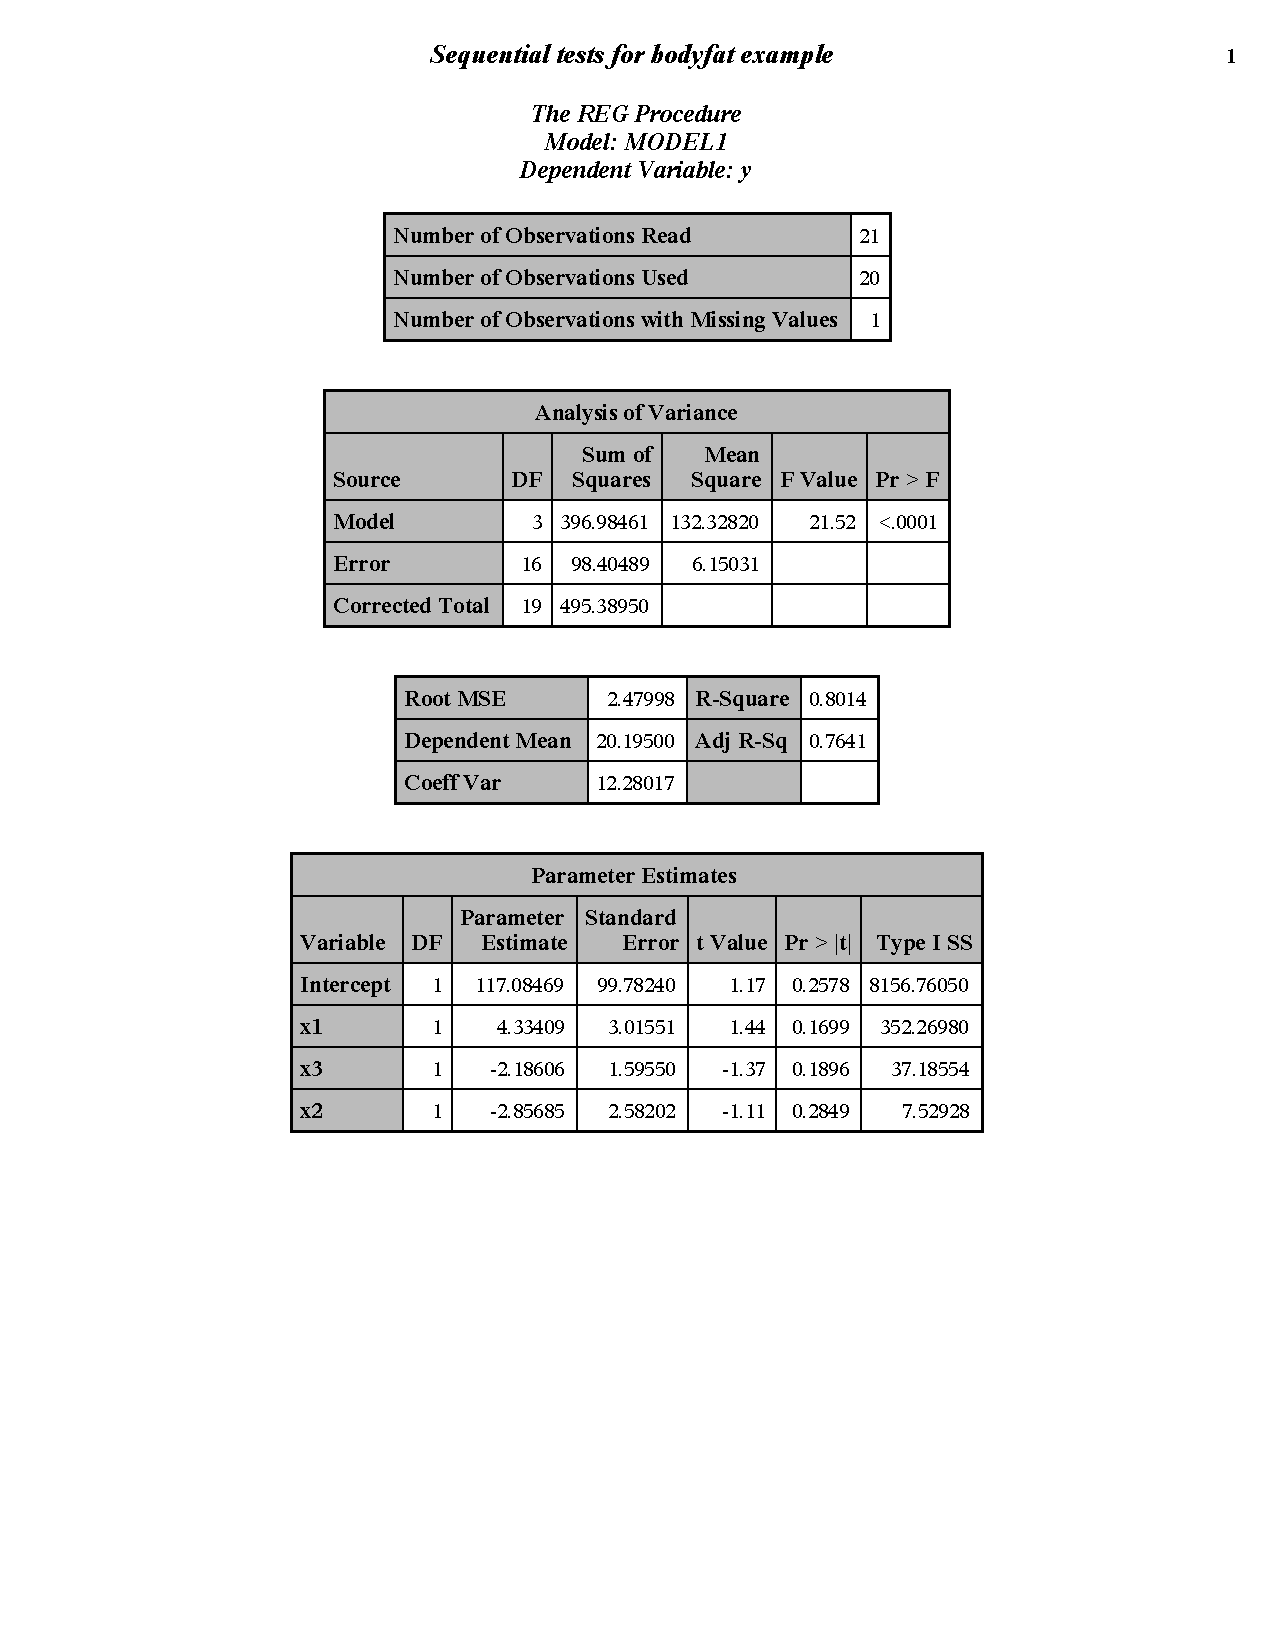
\includegraphics[page=1,scale=0.7,trim= 10mm 70mm 10mm 10mm]{bodyfatexampletypeI}
\end{center}

Let`s label the Type I SS in terms of extra regression sums of squares (R notation).

\newpage

Note: we will soon use proc glm for our model analysis and this gives even better output for type I sums of squares.  (The tests given for type I sums of squares use the \textit{full model} MS(E) rather than the full model MS(E) up to that point.  This test still works because MS(E) from each model is an unbiased estimate of $\sigma^2$.  The tests using the different MS(E) terms could give different results, but will usually agree.\\

\begin{small}
\begin{verbatim}
proc glm data=bodyfat;
   model y=x1 x3 x2;   
run;
\end{verbatim}
\end{small}

\begin{center}
\includegraphics[page=2,scale=0.7,trim= 10mm 80mm 10mm 0mm]{bodyfatexampletypeIglm}
\end{center}

\newpage

\textbf{A linear regression example with a quadratic explanatory variable:}\\
Data was collected on 5 kilometer run times.  The variables collected were age, sex, and pace.\\
\begin{small}
\begin{verbatim}
                  Obs    age    sex      race       pace

                    1     28     M     16.6833    5.38333
                    2     39     M     16.9500    5.46667
                    3     41     M     17.1333    5.51667
                    4     42     M     17.4000    5.61667
(abbreviated)     ...    ...   ...         ...        ...
                  157     52     F     46.8833    15.1000
                  158     10     F     53.6000    17.2667
                  159     10     F     53.6167    17.2667
                  160     81     M     54.3167    17.5000

\end{verbatim}
\end{small}

\begin{center}
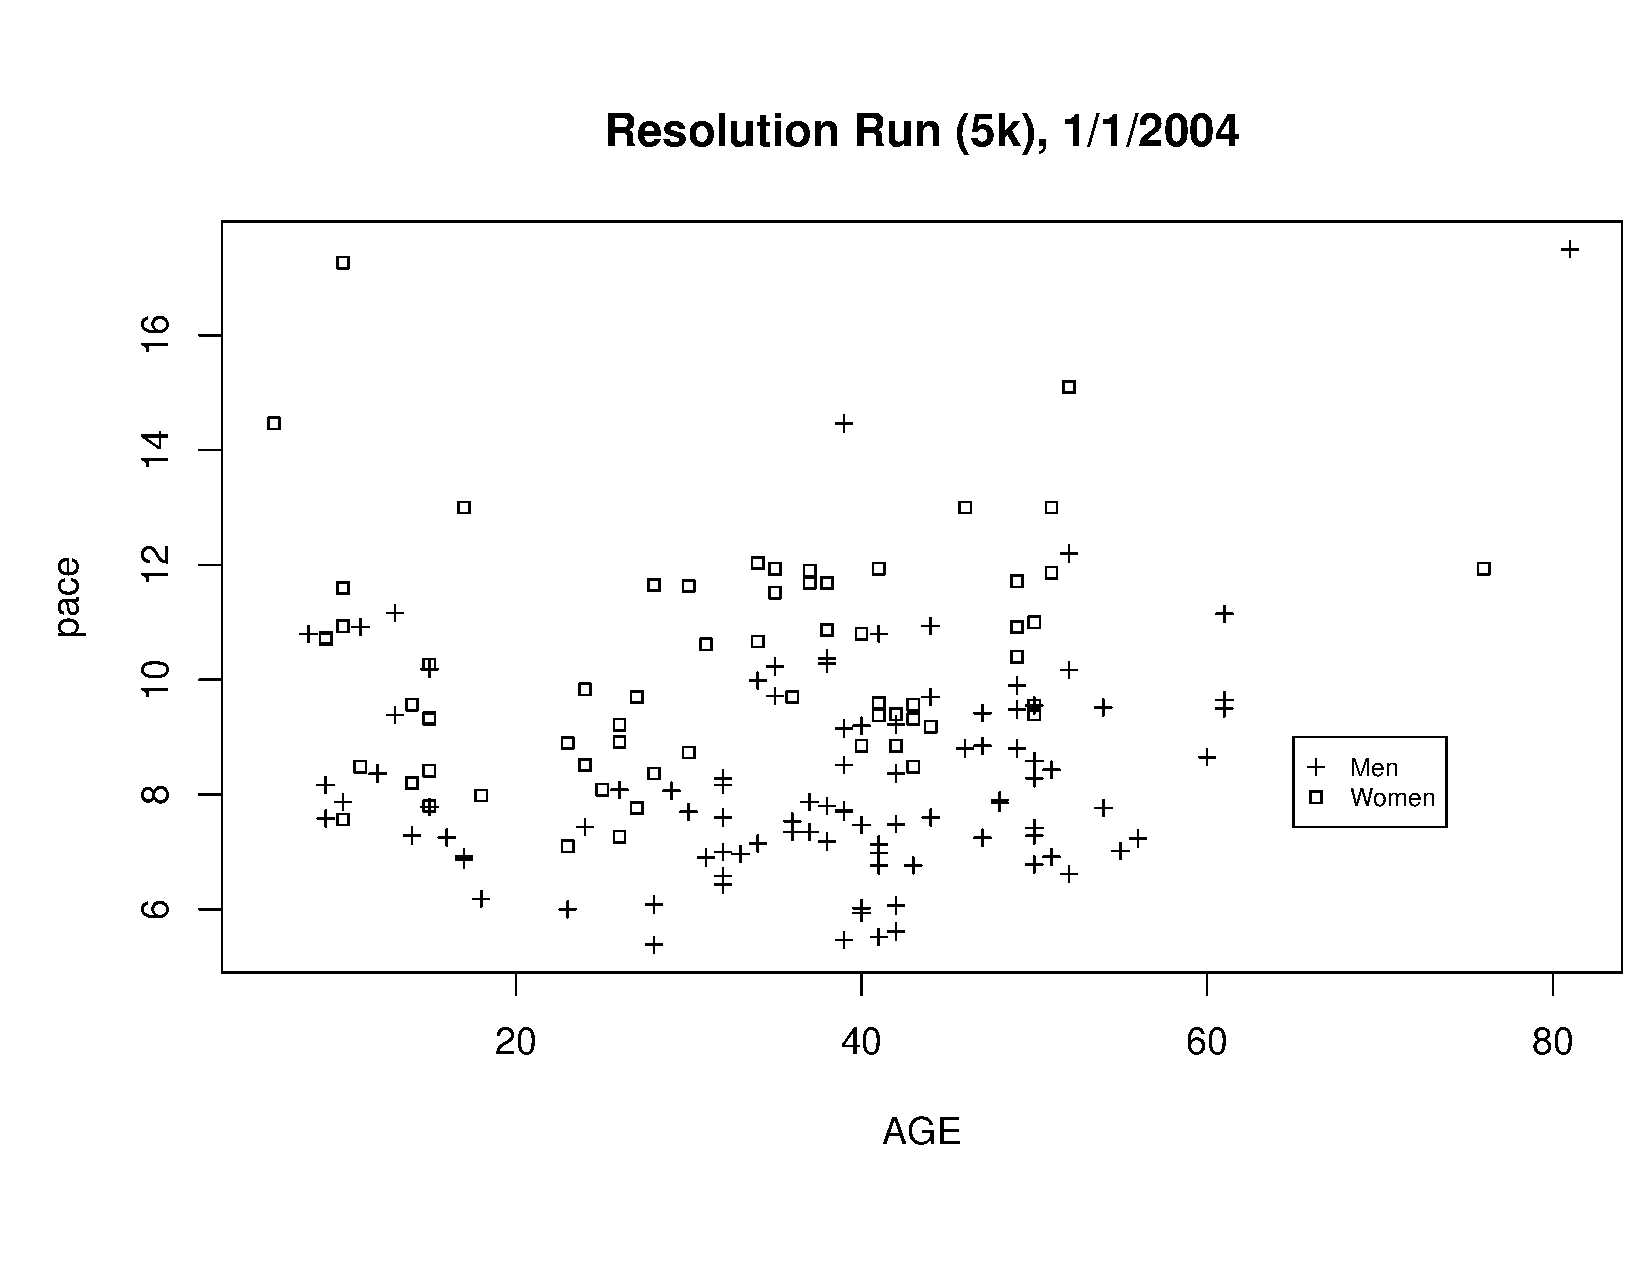
\includegraphics[height=3in,width=3in]{res5k_nomodel}
\end{center}

Quadratic model for pace ($Y$) as a function of age ($x$):
$$ Y_i = \beta_0 + \beta_1 x_i + \beta_2 x_i^2 + E_i \ \ \mbox{ for }i=1,\ldots,160$$
where $E_i \iid N(0,\sigma^2)$.\\~\\
Question: What does $\sigma^2$ represent in the model?\\~\\~\\~\\
Question: What do the parameters mean, i.e. what is their interpretation?

\newpage
 
We may want to compare this model with a SLR model 
$$ Y_i = \beta_0 + \beta_1 x_i + E_i \mbox{ for }i=1,\ldots,160$$
Question: How can we compare the two models?\\~\\~\\~\\

\begin{small}
\begin{verbatim}
/* age2 defined in data step as age*age */ 
PROC REG;
   MODEL pace=age;      
   MODEL pace=age age2/ss1 covb;
RUN;
\end{verbatim}
\end{small}
\begin{large}
\begin{verbatim}
                               Model: MODEL1
                           Analysis of Variance
 
                                   Sum of          Mean
 Source                  DF       Squares        Square   F Value   Pr > F
 Model                    1       1.09650       1.09650      0.22   0.6396
 Error                  158     786.99821       4.98100                   
 Corrected Total        159     788.09472                                 

           Root MSE              2.23182    R-Square     0.0014
           Dependent Mean        9.12063    Adj R-Sq    -0.0049

                        Parameter       Standard
   Variable     DF       Estimate          Error    t Value    Pr > |t|
   Intercept     1        8.92271        0.45724      19.51      <.0001
   age           1        0.00564        0.01203       0.47      0.6396

                               Model: MODEL2
                           Analysis of Variance
 
                                   Sum of          Mean
 Source                  DF       Squares        Square   F Value   Pr > F
 Model                    2     113.64500      56.82250     13.23   <.0001
 Error                  157     674.44972       4.29586                   
 Corrected Total        159     788.09472                                 

           Root MSE              2.07265    R-Square     0.1442
           Dependent Mean        9.12063    Adj R-Sq     0.1333
\end{verbatim}
\end{large}

\newpage

\begin{large}
\begin{verbatim}

                   Parameter     Standard
  Variable   DF     Estimate        Error  t Value  Pr > |t|    Type I SS
  Intercept   1     11.78503      0.70216    16.78    <.0001        13310
  age         1     -0.19699      0.04113    -4.79    <.0001      1.09650
  age2        1      0.00294   0.00057380     5.12    <.0001    112.54850

										Covariance of Estimates 
	Variable        Intercept     age           age2 
	Intercept       0.4930258    -0.0265145     0.0003209 
	age            -0.0265145     0.0016921    -0.0000227 
	age2            0.0003209    -0.0000227     0.0000003 

\end{verbatim}
\end{large}

\begin{center}
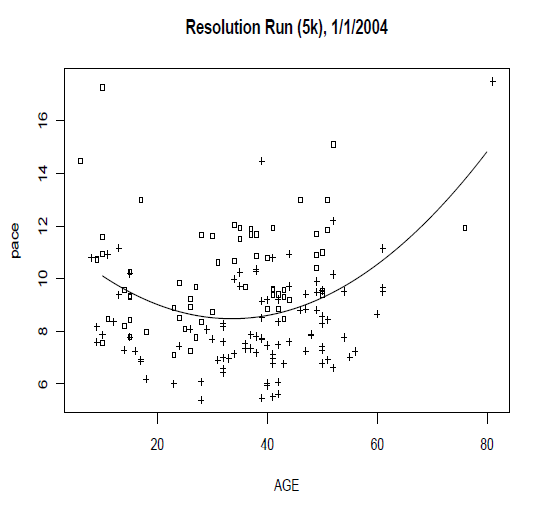
\includegraphics[scale=0.5]{res5k_quadratic}
\end{center}
Fitted models are:
$$\text{Model 1: } \hat\mu(x)=8.923 + 0.0056 age$$
$$\text{Model 2: } \hat\mu(age) = 11.785 - 0.197 age + 0.00294 age^2$$

\begin{eqnarray*}
F & = & \frac{R(\beta_2|\beta_0,\beta_1)}{MS(E)_{full}} \\
  & = & \frac{(SS(R)_{full}-SS(R)_{red})/1}{MS(E)_{full}} \\
  & = & \frac{(113.6-1.1)/1}{4.3} \\
  & = & \frac{(SS(E)_{red}-SS(E)_{full})/1}{MS(E)_{full}} \\
  & = & \frac{(787.0-674.4)/1}{4.3} = 26.2 \\
  & = & \left(\frac{\hat\beta_{ 2}}{SE}\right)^2 = (5.12)^2\\
\end{eqnarray*}
with $F(0.05,1,157)=3.90$.  Since $26.2 > > 3.9,$ we reject that the linear model is appropriate when compared to the quadratic model.  This is the same test as the t-test for age2!

